%=========================================================================
% (c) Michal Bidlo, Bohuslav Křena, 2008
\setcounter{secnumdepth}{4} % cislovani nadpisu do hloubky

\chapter{Úvod}
\label{chapter:1}

V současné době se technologie ve všech odvětvích stále posouvá a~není tomu jinak ani u~prohlížení fotek a~videí. V současné době i~takto nahrané informace pomocí digitálních zařízení je trend dále posouvat a~zvyšovat tak zážitek ze zaznamenané události. Díky tomuto trendu si už nevystačíme s ``klasickými''  přehrávači, popř. prohlížeči videí, nebo fotografií. Díky sférickým 360 stupňovým kamerám, je dnes možné zaznamenat video o~srovnatelné velikosti jako u dnes běžného telefonu, ale s~mnohem větším objemem informací, které se ale nedají srozumitelně přehrát v~klasických přehrávačích. Ruku v ruce se sdílením takových dát, je velice výhodné takový prohlížeč nabídnout jako webovou verzi, aby i~jiní uživatelé mohli svá takto natočená videa přehrávat popř. sdílet. Důkazem toho je rozmach multimediálního obsahu na internetu, kdy samotný jazyk HTML pro prezentaci webových stránek dříve nenabízel přímou podporu videí, což se změnilo příchodem nové verze HTML5. Některé portály jako např. Youtube již dnes začíná nasazovat do svého prohlížení videí jeho rozšířené sférické verze, což tedy potvrzuje tento trend. Tato práce má za cíl takové prohlížení posunout ještě dál.


Následující práce se věnuje implementaci webového prohlížeče panoramatických snímku a videí v různých módech, ve kterých je video interpretováno. Cílem je tedy navrhnout a zrealizovat řešení, aby uživatel po natočení videa dále nepotřeboval k přehrání např. sférického videa v režimu rybího oka specifický program, který by video musel nejprve překonvertovat. To stejné se týká i~panoramatických snímku a~videí v equirectangulárním zobrazení.  


Další inovací v prohlížení videí je přidání některých dat, které v běžném prohlížení není k dispozici. Např. informace o světových stranách ve vztahu k obrázku, či videu popřípadě údaje o velikosti zorného pole v daném kontextu prohlížení až po dodatečná metadata v~panoramatických obrázcích, které jsou vhodné např. k~tomu, aby autor obrázku mohl popsat jeho zajímavé částí popřípadě blíže popsat zachycenou scénu.
\newline

Samotná práce je členěna do šesti částí. V kapitole \nameref{chapter:2} se budu věnovat nastínění všech použitých technologií nutných pro pochopení problematiky, se kterými se bude pracovat v následujících kapitolách. O návrhu řešení pojednává kapitola \nameref{chapter:3}, na kterou navazuje implementační část \nameref{chapter:4}. Otestování správného návrhu a implementace se zabývá kapitola s názvem \nameref{chapter:5}. V poslední části práce \nameref{chapter:6} jsou prezentovány dosažené výsledky a možnosti dalšího rozšíření.

%=========================================================================


\chapter{Webové technologie prohlížeče}
\label{chapter:2}

\section{HTML5}

Jazyk HTML (HyperText Markup Language) je značkovací jazyk určený pro popis webových stránek. Vychází z univerzálního značkovacího jazyka SGML (Standard Generalized Markup Language). V současné době aktuální verzi  jazyka HTML je jeho již pátá verze -  HTML5. Nová verze HTML přináší zásadní vylepšení, nové funkce a možnosti, které jsou nezbytné pro návrh a implementaci webového prohlížeče. 

Pro návrh samotného programu je nezbytná podpora multimédií – tedy audio a video, v neposlední řádě také plátno canvas sloužící pro práci s grafikou.



\subsection{Video}
Dříve nebylo možné do webových stránek vložit video tak jako dnes. K tomuto účelu bylo využíváno různých zásuvných modulů třetích stran a do webových stránek se video vkládalo např. jako objekt. Nejvíce rozšířeným přehrávačem videí a tedy jakási náhrada za podporu videí, kterou tehdy HTML nemělo, se v širším spektru stal Adobe Flash, který funkci přehrávače plní v menší míře až doposud, avšak je již zastíněn efektivnějším řešením, a to právě HTML5.

Nový prvek v HTML5 vytvořený k tomuto účelu je \texttt{<video>}. Byl navržen tak, aby mohl být použit bez detekčních skriptů na stránce. V elementu videa je možné nastavit více souborů s videem a dle podpory si daný prohlížeč vybere jim podporované video. V případě, že by prohlížeč prvek videa nepodporoval, bude jej ignorovat. Nastavení více zdrojů videa s odlišnými kodeky lze pomocí elementu \texttt{<source>} uvnitř páru elementů \texttt{<video>...</video>}. Jakmile prohlížeč narazí na \texttt{<video>}, podívá se, zdali je přítomen atribut \texttt{src}, v opačném případě začne procházet jeden element \texttt{<source>} po druhém a bude hledat právě takový, který umí přehrát.

Aby bylo možné ovládat video dynamicky pomocí kláves nebo myší, bude nutné využít DOM (Document Object Model). Jedná se o stromovou strukturu dokumentu, kterou si prohlížeč sestavuje po načtení webové stránky. Všechny elementy webové stránky jsou interpretovány v DOM jako objekt Některé značky se v DOM vytvoří, aniž by byly ve zdrojovém kódu zapsány. Obecně platí, že pomocí objektového modelu je díky javascriptu možné tuto stromovou strukturu dále upravovat a rozšiřovat. 

%=========================================================================
\newpage

\subsubsection{Stavy načítání a přehrávání videa}
Další velice důležitou částí je načítáni videa a jeho ověření, zdali  je již video připraveno k přehrání. K ověření dostupnosti videa lze použít jeden ze síťových stavů elementu pomocí stavového atributu \texttt{networkState}, popřípadě přímo zjišťovat připravenost videa pomocí atributu \texttt{readyState}, vracející jeden z následujících stavů, podle kterých se můžeme dále při přehrávání řídit a přizpůsobit tomu běh programu. Jednotlivé konstanty nabývají hodnot od 0 do 4 a dle hodnot rozlišujeme:


\begin{itemize}
	\item \texttt{HAVE\_NOTHING } (ekvivalentní hodnotě 0) \newline
	 - nastane v situaci, kdy zdrojové video není dostupné, nebo žádná data pro aktuální přehrávanou pozici \newline - koresponduje také s návratovou hodnotou síťové metody \texttt{networkState()}, když její návratová hodnota je rovna 0, což odpovídá konstantě \texttt{NETWORK\_EMPTY}
	\item \texttt{HAVE\_METADATA} \newline
		-  základní data o zdroji se podařilo získat a zdroj je tedy považován jako dostupný. Zatím ale ještě není dostatek dat, aby bylo možné začít s přehráváním. V tomto stavu jsou k dispozici jen data popisující přehrávány subjekt, jako délka, šířka, dekódovaní apod. Dochází k vyvolání události \texttt{loadedmetadata}
	\item \texttt{HAVE\_CURRENT\_DATA }\newline
		- data pro bezprostřední začátek přehrávání jsou připravena, ale video ještě není načteno dál za tuto pozici. Přehrávání může dostat do stavu \texttt{HAVE\_METADATA}, nebo následující data videa již nejsou k dispozici.
	\item \texttt{HAVE\_FUTURE\_DATA}\newline
		- data pro přehrávání jsou připravena pro současnou i nadcházející pozici. V případě, že by bylo video dosáhlo takového stavu poprvé, bude vyvolána událost \texttt{canplay}.
	\item \texttt{HAVE\_ENOUGH\_DATA}\newline
		- data připravena pro aktuální a nadcházející pozice pro plynulé přehrání. Dochází k vyvolání události \texttt{canplaythrough}
\end{itemize}

Mimo stavy načtení videa jsou tu i stavy indikující, co přesně se právě děje s videem po jeho načtení. Tyto stavy se hodí k dotazování elementu \texttt{<video>} pomocí DOMu např. pro tvorbu vlastního specifického ovládání videa, nebo pro zahrnutí interakce s myší.



\begin{itemize}
	\item \texttt{playing} - video se aktuálně přehrává, atribut \texttt{paused} je nastaven na \texttt{false}	
	\item \texttt{waiting} - přehrávání videa je pozastaveno	
	\item \texttt{ended} - přehrávání videa doběhlo nakonec
	\item \texttt{canplaythrough} - tato událost říká, že je možné video přehrát až do konce bez nutnosti video zastavit k dalšímu načítání. Tohoto stavu může dosahnout jen v případě, že stavový atribut \texttt{readyState} je roven \texttt{HAVE\_ENOUGH\_DATA}.
	
\end{itemize}

%=========================================================================
\newpage

\subsubsection{Atributy videa}
Důležité atributy pro manipulaci s videem a nastavením.



\begin{description}
	\item[src] - jedná se o atribut, do kterého se definuje zdrojové adresa videa jako URL, které se má zobrazit. Používá se zejména v situaci, kdy je k dispozici právě jedna verze videa.
	
	\item[autoplay] - jedná se atribut typu \texttt{bool}. V případě, že je \texttt{true}, spustí se přehrávání média automaticky jakmile je vše připraveno. Uvedení názvu atributu do elementu samotného je již dostačující informace o tom, co se bude dít s videem. Tedy bude tato hodnota typu \texttt{bool} považována jako \texttt{true}, jinak \texttt{false}.	
	
	\item[poster]  - Slouží k vystihnutí obsahu daného videa. Ještě než začne samotné přehrávání, je možné jako první snímek videa zvolit obrázek zadaný cestou. V~případe, že tento atribut nebude vyplněn, HTML automaticky zvolí jeden z prvních neprázdných rámců.
	
	\item[loop]  - jedná se atribut typu \texttt{bool}, který začne po dosažení konce videa s přehráváním videa opět od začátku. Tato operace se provádí v nekonečné smyčce.

	\item[width] - šířka přehrávače v pixelech.
	
	\item[height] - výška přehrávače v pixelech.

	\item[paused] - atribut videa typu \texttt{bool}. Indikuje, zdali se video přehrává či nikoliv.

	\item[controls] - jedná se opět o atribut typu \texttt{bool}, který říká, aby prohlížeč použil vlastní ovládací prvky pro video. Ovládací prvky se dají také vytvořit a přizpůsobit velice snadno díky DOMu.
 	
 	\item[preload]  - tímto říkáme, jakou část videa by měl webový prohlížeč načíst ihned po načtení stránky. Tento atribut nabývá jednou ze tří hodnot:
	 	\begin{itemize}
	 		\item \texttt{none} - nebude načítat nic, výhodné v případě, kdy je potřeba minimalizovat vytížení pásma	 		
	 		\item \texttt{metadata} - načte pouze metadata daného videa - základní údaje o jeho délce apod.
	 		\item \texttt{auto} - sám zvolí, co přesně udělá 
	 	\end{itemize}
\end{description}

%=========================================================================
\newpage

\subsubsection{Metody videa}
Jelikož pomocí DOM je možné upravovat vlastnosti elementu \texttt{<video>}, tak jsou tedy nutné metody k ovlivnění jeho atributů, aby bylo možné s přehráváním videa manipulovat.

\begin{description}
	\item[\texttt{play()}] - metoda sloužící k nastavení atributu \texttt{paused} na \texttt{false}, pokud video již skončilo, začne je přehrávat od začátku.
	\item[\texttt{pause()}] - metoda sloužící k nastavení atributu \texttt{paused} na \texttt{true}, tím dojde k pozastavení videa
	\item[\texttt{canplaytype()}] - metoda sloužící k ověření, zdali webový prohlížeč dokáže video daného typu přehrát. Metoda vrací jednu z následujících hodnot:
	 	\begin{itemize}		
			\item \texttt{""} - pokud by metoda vrátila prázdný řetězec, video prohlížeč nedokáže přehrát.
			\item \texttt{maybe} - prohlížeč si není zcela jist, zdali dokáže formát přehrát.
			\item \texttt{probably} - daný formát videa dokáže prohlížeč přehrát s vysokou pravděpodobností.
		\end{itemize}
	\item[\texttt{load()}] - všechny data videa se načtou znovu, čímž dojde ke zrušení všech akcí a současných dat, které byly doposud staženy a načteny. Poté se vše zavolá a načte znovu následujícím způsobem:
	 	\begin{enumerate}
			\item Nejprve dojde k inicializaci, kdy \texttt{readyState} je nastaven na \texttt{HAVE\_NOTHING} a  nastaví i příslušný síťový atribut \texttt{networkState} na \texttt{0}, \texttt{seeking} je nastaven na \texttt{false}, \texttt{paused} je nastaven na \texttt{true}, vše ostatní je prázdné, nebo nula	
			
			\item vybere se zdroj z atributu \texttt{src} nebo \texttt{<source>}, dále je vyvolána událost \texttt{loadstart} a dochází ke stažení metadat videa
			
			\item jakmile jsou metadata stažena, nastaví se zakladní vlastnosti videa - šířka, výška, délka a \texttt{readyState} je nastaven na \texttt{HAVE\_METADATA} a spolu s tím je vyvolána událost \texttt{loadedmetadata}
			
			\item Jakmile je \texttt{readyState} větší nebo roven \texttt{HAVE\_FUTURE\_DATA} je vyvolána událost \texttt{canplay} a \texttt{loadeddata}
			
			\item dojde ke spuštění přehrávání. Je vyvolána událost \texttt{play} a \texttt{playing}, atribut \texttt{paused} nastaven na \texttt{false}
		\end{enumerate}
\end{description}


%=========================================================================
\newpage

\subsection{Plátno}

Jak již bylo avizováno výše, plátno, neboli element \texttt{<canvas>} slouží v HTML5 pro vykreslení grafů. herní grafiky, obrazů bitmap apod. Díky elementu \texttt{<canvas>} lze vykreslovat i náročnější grafické objekty za pomocí WebGl. V HTML5 slouží tedy především k vykreslení 2D prvků pomocí Javascriptu. Plátno je párový  element, přesto se mezi párové tágy zdánlivě nic nevykresluje, celý obsah je skryt. Takový obsah se nazývá tzv. \textit{fallback content} a je zobrazen v případě chyby, nebo prohlížečům, které tento element HTML5 nepodporují.

Plátno je bezpochyby nejdůležítější částí pro realizaci celé práce. Bude pro vyobrazení používat především \texttt{<video>}, z kterého bude číst data a využije tedy element video jak zdroj. Díky DOM pak dokážeme s objektem snadno manipulovat. Díky elementu \texttt{<canvas>} jsme tedy schopni získat kontext Javascriptového API - WebGl a díky němu schopni pracovat na úrovni grafické karty.

\subsubsection{Atributy plátna}
Canvas má pouze dva atributy a těmi jsou \texttt{width} a \texttt{height} pro nastaveni šířky a výšky plátna. Je možné nastavit výšku a šířku pomocí kaskádových stylů, avšak tato možnost není doporučována, protože by mohlo dojít k nežádoucí deformaci obsahu. Při změně velikosti bitmapy pomocí atributů dojde pouze ke změně velikosti dané bitmapy, změna kaskádovými styly ale změní velikost obsahu celé bitmapy a tím tedy dojde ke zkreslení.

\subsubsection{Použití a práce s plátnem}
Použit plátno lze pomocí rozhraní \texttt{HTMLCanvasElement}, které slouží pro přístup k jeho vlastnostem a metodám. Přístup k objektu \texttt{HTMLCanvasElement} lze pomoci standardní javascriptové metody \texttt{getElementById()} v případě, že je v tágu \texttt{<canvas>} nastaven atribut \texttt{id}, nebo lze objekt získat pomocí metody \texttt{querySelector("canvas")}.

Po získání objektu plátna lze dále s elementem manipulovat pomocí dvou metod (počet volání dané metody vrátí pokaždé ten stejný objekt):
	 	\begin{itemize}		
			\item \texttt{ toDataURL([type[,quality]])}\newline
			 - vrací URL adresu aktuálního obrázku v elementu \texttt{<canvas>}. Metoda může a nemusí mít nějaké argumenty. První argument, v případě že je zadán, rozhoduje jaký bude navrácen výsledný typ obrázku. Pokud nezadáme žádný argument, tak jako výchozí formát obrázku bude automaticky zvolen \textit{image/png}. Výsledná adresa URL bude vrácena jako řetězec.
			\item \texttt{getContext(contextId[, ... ])}\newline
			 - metoda vrací referenci na daný objekt aplikačního rozhraní, díky kterému bude možné kreslit na plátno. Pokud by kontext pro daný argument nebyl podporován prohlížečem, návratová hodnota bude \texttt{null}. Typ aplikačního rozhraní je vybrán na základě argumentu metody:
			 \begin{itemize}
			 	\item  \texttt{\textbf{"2d"}} - vrací objektové rozhraní \texttt{CanvasRenderingContext2D}, kterí slouží pro kreslení grafických primitiv.
			 	\item \texttt{\textbf{"webgl"}} - pokud tuto funkci prohlížeč podporuje, bude navrácen objekt \newline \texttt{WebGLRenderingContext}. 
			 \end{itemize}
		 
 
		\end{itemize}

%=========================================================================
\newpage


%=========================================================================



\section{GLSL}
\textbf{GLSL} (Open\textbf{GL} \textbf{S}hading \textbf{L}anguage) - jedná se o jazyk pro psaní shaderů \footnote{Jedná se o programy řídící vykreslování na grafické kartě}. Jazyk vychází z jazyka C a také proto je mu svojí syntaxí velice podobný. Základní konstrukce každého programu je v zásadě úplně stejná jako v jazyku C, každý program musí obsahovat hlavní funkcí \texttt{main()} bez jakýkoliv parametrů a návratových hodnot. V hlavní funkci programu jsou vyhrazeny proměnné se speciálním významem, jako např. \texttt{gl\_Position}, kterou nastavujeme  pozici vrcholu ve vertex shaderu, nebo \texttt{gl\_FragColor} pro nastavení barvy ve fragment shaderu.

\subsection{Vertext shader}
Jedná se o program v jazyce GLSL, který je pro prováděn pro každý vstupní vrchol zadané geometrie. Každá souřadnice vrcholu je dále přepočítána do tzv. \textit{clipspace}, což je souřadný systém pro vykreslování do plátna. V případě, že by některé souřadnice byly mimo hranice souřadného systému, budou oříznuty a vykreslovat se nebudou. Hranice \textit{clipspace} jsou definovány pro každou ze souřadnic \texttt{x},\texttt{y}, \texttt{z} intervalem \texttt{<-1,1>}. Vertex shader může sám ovlivnit souřadnice vrcholů, textur popř. normálových vektorů a barev. Při zpracování vrcholů není známa topologie zpracovávaného objektu, protože nejsou dostupné informace o sousedících vrcholech.

\subsection{Fragment shader}
Je program - označovaný taktéž jako \textit{pixel shader}, který je volán pro každý pixel vykreslované scény. Jeho úkolem je výpočet barvy každého pixelu a díky tomu lze s takto získanou barvou  dále pracovat. Barva je získána jako čtyřsložkový vektor, první tří složky tvoří paletu RGB, poslední čtvrtá složka tvoří $\alpha$ kanál \footnote{Složka pixelu udávající jeho průhlednost}. V případě vykreslování složitějších objektů umožňuje GLSL automaticky body geometrie interpolovat, tedy automaticky získat pixel dané geometrie, aniž by musel být každý samostatně definován. Ukázka interpolace je demonstrována na obrázku \ref{img:1}.

 \newpage
 
 
\begin{figure}[h]
	\label{img:1}
	\centering
	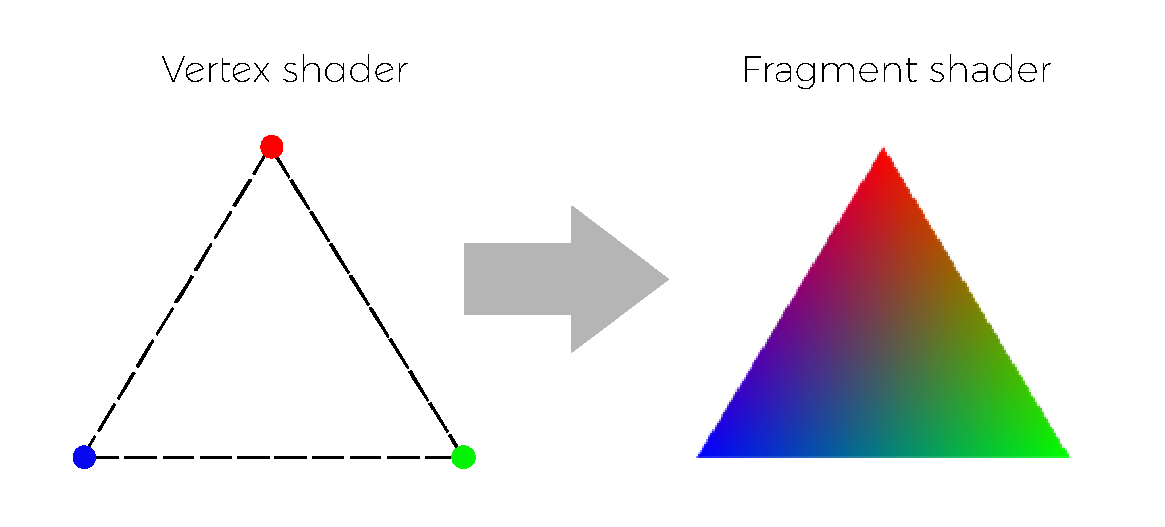
\includegraphics[scale=1.0,angle=0,width=1.0\linewidth]{inter}
	% 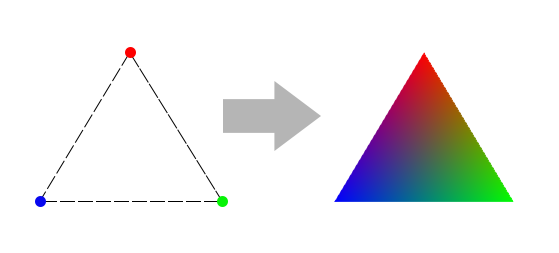
\includegraphics[scale=1.0,height=2.5in,angle=0]{interpolace.png}
	\caption{Ukázka interpolace hodnot mezi vertex a fragment shaderem.}
	\label{fig:inter}
\end{figure}
 



\subsection{Typy proměnných}
Předávání hodnot v globálních
\begin{itemize}
	\item 
\end{itemize}
\newpage


 

\section{WebGL}
WebGL (\textbf{Web} \textbf{G}raphics \textbf{L}ibrary) je javascriptové aplikační rozhraní, které slouží pro nativní vykreslování 2D a 3D interaktivní grafiky přímo z webového prohlížeče. K samotnému běhu WebGL není potřeba žádných dodatečných knihoven, nebo zásuvných modulů, protože je v tomto ohledu využívána přímo grafická karta. Program WebGL se v zásadě skládá z více jazyků, přičemž každý mů svůj vlastní účel a je nutné je používat dohromady. Jedním z nich je javascript, druhý je jazyk GLSL. V jazyce GLSL jsou napsány dva programy - vertex shader a fragment shader. Oba programy kompiluje ovladač grafické karty do kódu, který je poté vykonáván přímo na grafické kartě. Vertex shader i fragment shader mohou být předávány jako řetězce, takže manipulace s nimi je díky tomu značně zjednodušena. Velkou výhodou WebGL je integrace s DOM tudíž od automatické správy pamětí přes zpracování událostí až po jednoduché načítání bitmapy přímo v prostředí prohlížeče apod..

K samotnému vykreslení je použit již výše zmíněný element HTML5 \texttt{<canvas>}.

V současné době je oficiálně vydána verze WebGL 1.0, která je založeno na OpenGL ES 2.0. Doposud se jedná o jedinou stabilní verzi. OpenGL ES\footnote{OpenGL for Embedded Systems} je zjednodušená verze OpenGL, která eliminuje většinu vykreslovacích pipeline. Tato verze je především určena pro menší vestavěné systémy. Dalším rozšířením WebGL bude verze 2.0, která se stále nachází ve vývoji. Bude založena na OpenGL ES 3.0 přinášející velká vylepšení v zobrazování 3D grafiky - zejména textur, akceleraci vizuálních efektů, novou verzí jazyka GLSL s plnou podporu desetinných a celočíselných operací apod.

\subsection{Vykreslování primitiv}
K vykreslení nějakého grafického prvku jsou potřeba v zásadě jen dvě věci - vrcholy přepočítané do tzv. \textit{clipspace} a jemu přiřazené odpovídající barvy. Jak pro vrcholy tak pro barvy slouží jiný GLSL shader. K vyobrazení objektu používá WebGL tří základní primitiva - vykreslení samotných bodů, čar nebo trojúhelníku. Vše funguje tak, že zadaný bod, kterému budeme chtít přiřadit barvu, se načte do odpovídající speciální globální proměnné ve vertex shaderu, tam se daná hodnota přepočítá do intervalu \texttt{<-1,1>} pro všechny jeho osy a vzniklá hodnota se uloží na grafické kartě. Počet bodu záleží na primitivu, které vykreslujeme. Pokud se tedy jedná o bod, stačí pouze jeden bod ve vertex shaderu, pokud se jedna o čáru tak dvě popř. trojúhelník, tak trojice bodů. GPU\footnote{Graphic Processing Unit - grafický procesor} poté zjistí, které pixely korespondují s vykreslovaným primitivem a pro každý takový pixel zavolá fragment shader. 



%=========================================================================

\chapter{Návrh řešení: sem nějakej zajimavej název kapitoly}
\label{chapter:3}



%=========================================================================

\chapter{Samotná implementace prohlížeče: aby ten nadpis zaujmul}
\label{chapter:4}

Pravidla \cite{Pravidla}. 

\chapter{Testování}
\label{chapter:5}


\chapter{Závěr}
\label{chapter:6}

Závěrečná kapitola obsahuje zhodnocení dosažených výsledků se zvlášť vyznačeným vlastním přínosem studenta. Povinně se zde objeví i zhodnocení z pohledu dalšího vývoje projektu, student uvede náměty vycházející ze zkušeností s řešeným projektem a uvede rovněž návaznosti na právě dokončené projekty.

%=========================================================================
